% СПО ЛКС - облачные вычисления
% Пынькин Д.А. (с) 2011
\documentclass[ignorenonframetext, hyperref={pdftex, unicode}]{beamer}
\usepackage{beamerthemesplit}

\usetheme{Pittsburgh}
\usecolortheme{dolphin}

\usepackage[russian]{babel}
\usepackage[utf8]{inputenc}
\usepackage[T1]{fontenc}
\usepackage{ulem}
%\usepackage{html}

\usepackage{verbatim}

\usepackage{tikz}
\usetikzlibrary{positioning,arrows}

\title[СПОЛКС (http://goo.gl/32cTB)]{Системое программное обеспечение локальных компьютерных сетей}
\author{Денис Пынькин}
\date{2011 -- 2012}
%\institution[БГУИР]{Белорусский государственный университет информатики и радиоэлектроники}
%\logo{
\includegraphics[width=1cm]{logo-kafEVM.png}}


\subtitle{Облачные\\вычисления}

\begin{document}

\mode<all>{\begin{frame}
\titlepage
\begin{center}
e-mail: denis.pynkin@bsuir.by\\
\end{center}
\begin{center}
{\bfseries http://goo.gl/32cTB}

{\tiny СЧАСТЬЕ ДЛЯ ВСЕХ, ДАРОМ, И ПУСТЬ НИКТО НЕ УЙДЕТ ОБИЖЕННЫЙ!\\
(c)Стругацкие, Пикник на обочине}
\end{center}
\end{frame}
}

%
% Далее начинается сама презентация
%
\section{}

\begin{frame}{Определение}
	\begin{block}{Облачные вычисления (cloud computing)}
это модель обеспечения повсеместного и удобного сетевого доступа по требованию к общему пулу 
конфигурируемых вычислительных ресурсов (например сетям передачи данных,  серверам,  
устройствам хранения данных,  приложениям и сервисам -- как вместе,  так и по отдельности),  
которые могут быть оперативно предоставлены и освобождены с минимальными эксплуатационными 
затратами и/или обращениями к провайдеру.
	\end{block}
\end{frame}


\begin{frame}{Все еще определение}
Cloud computing -- тип Интернет-ориентированных вычислений, при котором использование IT ресурсов организацией имеет все перечисленные характеристики:

	\begin{itemize}
		\item Доступ к ресурсам:
		\begin{itemize}
			\item контролируется сущностью, при этом  ограничивает доступ к ресурсам для авторизованных пользователей;
			\item предоставляется через Интернет;
		\end{itemize}

	\item Ресурсы:
		\begin{itemize}
			\item предоставляются сервисным провайдером от имени организации;
			\item выделены для эксклюзивного использования организацией;
		\end{itemize}
	\item Данные:
		\begin{itemize}
			\item частные для организации и ее сотрудников;
			\item вводятся, собираются либо автоматически генерируются с помощью ресурсов;
		\end{itemize}
	\end{itemize}

\end{frame}

\begin{frame}{Базовые технологии}
	\begin{itemize}
		\item виртуализация (60-е);
		\item разделение времени (60-70-е);
		\item клиент-серверная модель (70-е);
		\item "коммунальные" вычисления (80-е);
		\item кластерные вычисления (60-е) и GRID (90-е);
		\item автономные вычисления (2001).
	\end{itemize}
\end{frame}


\begin{frame}{Для чего?}
	\begin{block}{Поставщику}
благодаря объединению ресурсов и непостоянному характеру потребления со стороны потребителей,  облачные вычисления позволяют экономить на масштабах,  используя меньшие аппаратные ресурсы,  чем требовались бы при выделенных аппаратных мощностях для каждого потребителя,  а за счёт автоматизации процедур модификации выделения ресурсов существенно снижаются затраты на абонентское обслуживание.
	\end{block}
\end{frame}

\begin{frame}{Для чего?}
	\begin{block}{Потребителю}
С точки зрения потребителя,  эти характеристики позволяют получить услуги с высоким уровнем доступности (англ. high availability) и низкими рисками неработоспособности,  обеспечить быстрое масштабирование вычислительной системы благодаря эластичности без необходимости создания,  обслуживания и модернизации собственной аппаратной инфраструктуры.

Удобство и универсальность доступа обеспечивается широкой доступностью услуг по и поддержкой различного класса терминальных устройств (персональных компьютеров,  мобильных телефонов,  интернет-планшетов).
	\end{block}
\end{frame}

\begin{frame}{Облачные роли}
	\begin{itemize}
		\item потребитель -- использует сервисы;
		\item провайдер -- предоставляет сервисы;
		\item аудитор -- проверяет сервисы от имени потенциального потребителя (например безопасность и приватность данных);
		\item брокер -- сущность, которая "договаривается" и управляет взаимоотношениями между потребителями и поставщиками сервисов (распределение нагрузки, агрегация сервисов);
		\item \sout{извозчик} провайдер линии связи (carrier) -- соединяет потребителя и поставщика сервиса (напимер ISP).
	\end{itemize}
\end{frame}



\begin{frame}{Характеристики}
	Обязательные характеристики облачных вычислений согласно NIST:

	\begin{itemize}
		\item Самообслуживание по требованию (On-demand self-service) -- предоставление необходимых ресурсов без необходимости взаимодействия человека с каждым провайдером;
		\item Универсальный доступ по сети (Broad network access);
		\item Объединение ресурсов (Resource pooling) -- физические и виртуальные ресурсы провайдера динамически (пере)распределяются между потребителями (+ прозрачность местоположения);
		\item Эластичность (Rapid elasticity) -- количество предоставляемых ресурсов;
		\item Учёт потребления (Measured service).
	\end{itemize}
\end{frame}

\begin{frame}{Сервисные модели}
	\center
	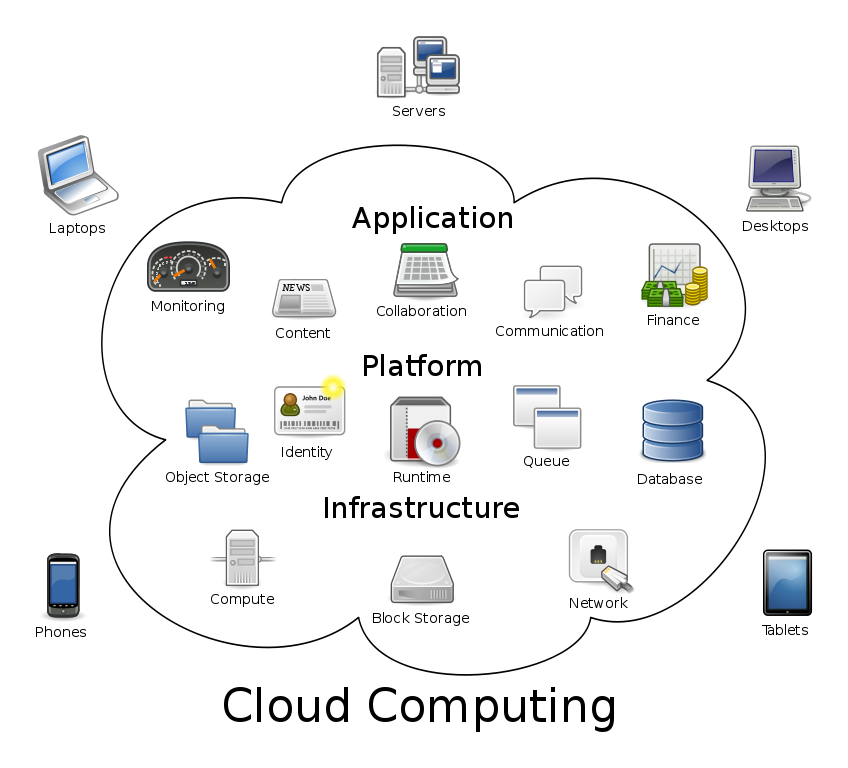
\includegraphics[width=0.8\textwidth]{Cloud_computing.png}
\end{frame}


\begin{frame}{Модели: SaaS}
	\begin{block}{Software as a Service}
		Программное обеспечение как услуга -- модель,  в которой потребителю предоставляется возможность использования прикладного программного обеспечения провайдера,  работающего в облачной инфраструктуре и доступного из различных клиентских устройств или посредством тонкого клиента,  например,  из браузера (например,  веб-почта) или интерфейс программы.

		\bigskip
		Контроль и управление основной физической и виртуальной инфраструктурой облака в том числе сети,  серверов,  операционных систем,  хранения,  или даже индивидуальных возможностей приложения (за исключением ограниченного набора пользовательских настроек конфигурации приложения) осуществляется облачным провайдером.
	\end{block}
\end{frame}

\begin{frame}{SaaS: характеристики/признаки}
	\begin{itemize}
		\item доступ к программному обеспечению, предоставляется удалённо по сетевым каналам и как правило через веб-интерфейс,  кроме того,  могут использоваться тонкие клиенты и терминальный доступ;
		\item программное обеспечение развёртывается в центре обработки данных в виде единого программного ядра,  с которым работают все заказчики;
		\item программное обеспечение предоставляется на условиях уплаты периодических арендных платежей;
		\item обслуживание и обновление программного обеспечения выполняется централизованно на стороне поставщика приложения,  предоставляемого как услуга (SaaS);
		\item стоимость технической поддержки обычно включается в арендную плату.
	\end{itemize}
\end{frame}

\begin{frame}{SaaS: варианты}
	\begin{itemize}
		\item Software as a Service (SaaS);
		\item Desktop as a Service (DaaS);
		\item Workspace as a Service (WaaS -- предоставление комплекта  SaaS, предназначенного для создания рабочего окружения)
		\item Database as a Service (DbaaS);
		\item Identity as a Service (IDaaS);
		\item Monitoring as a Service (MaaS).
	\end{itemize}

\end{frame}

\begin{frame}{Модели: PaaS}
	\begin{block}{Platform as a Service}
		Платформа как услуга -- модель,  когда потребителю предоставляется возможность использования облачной инфраструктуры для размещения собственных либо приобретенных приложений, которые используют ЯП, библиотеки, сервисы и утилиты, поддерживаемые провайдером.

		\bigskip
Контроль и управление основной физической и виртуальной инфраструктурой облака,  в том числе сети,  серверов,  операционных систем,  хранения осуществляется облачным провайдером,  за исключением разработанных или установленных приложений,  а также,  по возможности,  параметров конфигурации среды (платформы).
	\end{block}
\end{frame}

\begin{frame}{PaaS: характеристики}
	\begin{itemize}
		\item сервисы для разработки, тестирования, развертывания, хостинга и обслуживания приложений в интегрированной среде разработки;
		\item средства для создания Web-ориентированных пользовательских интерфейсов;
		\item архитектура с использованием мульти-аренды (Multi-tenant) -- масштабируемость,  отказоустойчивость,  виртуализация и безопасность;
		\item интеграция веб-сервисов и баз данных,  использование распространенных веб-стандартов,  возможность интеграции сервисов расположенных в частных сетях (SOAP, REST); 
		\item поддержка совместной работы команды разработчиков;
		\item аренда оборудования и оплата только тех ресурсов и сервисов,  которые необходимы.
	\end{itemize}
\end{frame}

\begin{frame}{Модели: IaaS}
	\begin{block}{Infrastructure as a Service}
Инфраструктура как услуга -- возможность использования облачной инфраструктуры для самостоятельного управления ресурсами обработки,  хранения,  сетей и другими фундаментальными вычислительными ресурсами,  например потребитель может устанавливать и запускать произвольное программное обеспечение,  которое может включать в себя операционные системы,  платформенное и прикладное программное обеспечение.

		\bigskip
		Контроль и управление основной физической и виртуальной инфраструктурой облака,  в том числе сети,  серверов,  типов используемых операционных систем,  систем хранения осуществляется облачным провайдером.
	\end{block}
\end{frame}


\begin{frame}{IaaS: варианты}

	\begin{itemize}
		\item Hardware as a Service (HaaS -- Оборудование (вычислительные мощности) как услуга);
		\item Communications as a Service (CaaS -- Коммуникация как Сервис) -- VoIP, IM, видеоконференции и др.;
		\item Infrastructure as a Service (IaaS) -- фактически IaaS является комбинацией SaaS,  HaaS, CaaS и иногда MaaS (Eucalyptus, OpenNebula, OpenStack, Nimbus и др.);

	\end{itemize}
\end{frame}


\begin{frame}{EaaS -- сферическое облако в вакууме?}
	\begin{block}{Everything as a service}
		концептуальная модель, включающая в себя элементы всех перечисленных решений.
		
		На данный момент полной её реализации не существует -- она по сути является идеалом для крупных облачных компаний, таких как Google и Microsoft.
	\end{block}
\end{frame}


\begin{frame}{Модели равёртывания}
	\begin{itemize}
		\item Частное облако (private cloud);
		\item Публичное облако (public cloud);
		\item Общественное облако (community cloud);
		\item Гибридное облако (hybrid cloud).
	\end{itemize}
\end{frame}


\begin{frame}{Частное облако}
инфраструктура,  предназначенная для использования одной организацией,  включающей несколько потребителей (например,  подразделений одной организации),  возможно также клиентами и подрядчиками данной организации.

\bigskip
Частное облако может находиться в собственности,  управлении и эксплуатации как самой организации,  так и третьей стороны (или какой-либо их комбинации),  и оно может физически существовать как внутри так и вне юрисдикции владельца.
\end{frame}


\begin{frame}{Публичное облако}
инфраструктура,  предназначенная для свободного использования широкой публикой. 

\bigskip
Публичное облако может находиться в собственности,  управлении и эксплуатации коммерческих,  научных и правительственных организаций (или какой-либо их комбинации). Публичное облако физически существует в юрисдикции владельца -- поставщика услуг.
\end{frame}

\begin{frame}{Общественное облако}
инфраструктура,  предназначенная для использования конкретным сообществом потребителей из организаций,  имеющих общие задачи (например,  миссии,  требований безопасности,  политики,  и соответствия различным требованиям).

\bigskip
Общественное облако может находиться в кооперативной (совместной) собственности,  управлении и эксплуатации одной или более из организаций сообщества или третьей стороны (или какой-либо их комбинации),  и оно может физически существовать как внутри так и вне юрисдикции владельца.
\end{frame}

\begin{frame}{Гибридное облако}
комбинация из двух или более различных облачных инфраструктур (частных,  публичных или общественных),  остающихся уникальными объектами,  но связанных между собой стандартизованными или частными технологиями передачи данных и приложений (например,  кратковременное использование ресурсов публичных облаков для балансировки нагрузки между облаками).
\end{frame}

\begin{frame}{Недостатки}
	\begin{itemize}
		\item приватность -- не все данные можно доверить стороннему провайдеру, тем более, не только для хранения, но и для обработки;
			\pause
		\item "отчетность" провайдера -- регулируется законами и правительственными организациями страны провайдера; 
			\pause
		\item далеко не каждое облачное приложение позволяет сохранить полученные результаты в удобном для пользователя виде на нужный носитель данных;
			\pause
		\item риск массовой потери данных многими пользователями из-за технического сбоя у поставщика облачных услуг;
			\pause
		\item потеря свободы пользователя и монополизм поставщика услуг: {\it ''жри, что дают''}.
			(В том числе при обновлениях -- например, при внедрении нового интерфейса, подписчикам придётся им пользоваться.
			\pause
		\item необходимость доступа к Интернету. 
	\end{itemize}
\end{frame}

\begin{frame}{''Cloud computing is a trap'' ?}
	\begin{block}{Richard Stallman:}
Использовать веб-приложения для своих вычислительных процессов не следует,  например,  потому,  что вы теряете над ними контроль. И это не лучше,  чем использовать любую проприетарную программу. Делайте свои вычисления на своём компьютере,  используя программы,  уважающие вашу свободу. Если вы используете любую проприетарную программу или чужой веб-сервер,  вы становитесь беззащитными. Вы становитесь игрушкой в руках того,  кто разработал это ПО.
	\end{block}
\end{frame}

\mode<all>{\begin{frame}{}
\Huge
\begin{center}
	Спасибо за внимание!
	\bigskip
	Вопросы?
\end{center}
\normalsize
\end{frame}
}

\end{document}
%Конец файла
